\section{Preliminaries}
\label{sec:background}

The following chapter provides an introduction to the field of Normalizing Flows. 
Section~\ref{sec:background_introduction_NF} discusses the basic concepts on which normalizing flows rely, namely the rule of change of variables, and how a flow can be used for density estimation and sampling. 
Consecutively, Section~\ref{sec:background_flow_layers} provides an overview of commonly applied flow layers and their properties.

\subsection{Introduction to Normalizing Flows}
\label{sec:background_introduction_NF}

Normalizing flows are a family of generative models that learn to transform a simple probability distribution like a Gaussian into a more complex distribution. 
Thereby, a characteristic of normalizing flows is that they are invertible such that the flow models a bijective mapping between the two distributions.
Initially proposed by \citet{NormalizingFlowsOriginalMathConcept}, normalizing flows have been popularized in the machine learning community by \citet{NormalizingFlowsFundamentals} in the context of variational inference, specifically to enable a more flexible posterior distribution, and by \citet{RealNVP} for density estimation, particularly on images. 

\subsubsection{Change of Variables}
To transform a (complex) probability density $p\left(\bm{z}^{(0)}\right), \bm{z}^{(0)}\in\mathbb{R}^{d}$ into a simpler, known distribution $p\left(\bm{z}^{(K)}\right)$, normalizing flows apply a sequence of invertible transformations $f_1,...,f_K:\mathbb{R}^d \to \mathbb{R}^d$ \cite{NormalizingFlowsOriginalMathConcept, NormalizingFlowsFundamentals}. These functions have to be differentiable and model a bijective mapping from $p\left(\bm{z}^{(0)}\right)$ to $p\left(\bm{z}^{(K)}\right)$, and reverse. Using the rule of change of variables, the likelihood of the input $\bm{z}^{(0)}$ can be expressed as follows:
\begin{equation}
	\label{eqn:related_work_change_of_variables}
	p(\bm{z}^{(0)}) = p(\bm{z}^{(K)}) \cdot \prod_{k=1}^{K} \left|\det \frac{\partial f_k(\bm{z}^{(k-1)})}{\partial \bm{z}^{(k-1)}}\right|
\end{equation}
where $\bm{z}^{(k)}=f_{k}(\bm{z}^{(k-1)})$. The second term on the RHS is the determinant of the Jacobian for $f_1,...,f_K$, and represents the change of volume modeled by the transformations. This part ensures that the probability mass overall remains unchanged for any possible transformation.

Intuitively, the transformations $f_1,...,f_K$ can be arbitrarily complex, and one could find a single transformation to model a bijective mapping for any two distributions \cite{Bogachev_2005, NormalizingFlowsOverview}. 
Therefore, flow-based models can represent any distribution $p\left(\bm{z}^{(0)}\right)$ if the transformations are complex enough \cite{NormalizingFlowsOverview2}.
However, finding the Jacobian for an arbitrary function is computationally expensive and not feasible, especially when the parameters of the flow should be learned. 
Thus, the transformations are often designed to allow efficient computation of its determinant. 
This is commonly achieved by choosing $f$ such that the Jacobian is a triangular matrix, as the determinant is then simply the multiplication of the Jacobian's diagonal:
\begin{equation}
    \det \frac{\partial f_k(\bm{z}^{(k-1)})}{\partial \bm{z}^{(k-1)}} = \prod_{i} \frac{\partial {f_k(\bm{z}^{(k-1)})}_i}{\partial \bm{z}^{(k-1)}_i}
\end{equation}
In conclusion, normalizing flows consist of transformations that are convenient to compute, invert and calculate the determinant of their Jacobian \cite{NormalizingFlowsOverview}.

\subsubsection{Density estimation and sampling}
A natural application of normalizing flows is density estimation by parameterizing the flow transformations: $f_k(\bm{z}^{(k-1)};\bm{\theta}_k)$ \cite{NormalizingFlowsOverview}. Given observed data $\mathcal{D}=\{\bm{z}_i\}_{i=1}^{M}$ from some unknown, complex distribution, we can perform likelihood-based estimation of the parameters by maximizing the data log-likelihood:
\begin{equation}
    \log p(\mathcal{D};\bm{\theta}) 
    = \sum_{\bm{z}^{(0)} \in \mathcal{D}} \log p(\bm{z}^{(0)}; \bm{\theta}) 
    = \sum_{\bm{z}^{(0)} \in \mathcal{D}} \left[ \log p(\bm{z}^{(K)}) + \sum_{k=1}^{K} \log \left|\det \frac{\partial f_k(\bm{z}^{(k-1)}; \bm{\theta}_k)}{\partial \bm{z}^{(k-1)}}\right| \right]
\end{equation}
The prior distribution $p(\bm{z}^{(K)})$ is chosen such that it allows fast density estimation and sampling itself. 
If needed, it can contain trainable parameters itself, such as the mean and the scaling.
Hence, a normalizing flow can be trained to model the dataset distribution via standard methods like stochastic gradient descend. 
In contrast to methods like \acp{VAE}, normalizing flows can use the exact likelihood as an objective and do not model a lower bound.

Once a flow sufficiently models a data distribution, a second common application is sampling. 
This can be done by sampling from the prior distribution, and apply the inverse transformations $f_1^{-1},...,f_K^{-1}$ in reverse order:
\begin{equation}
    \begin{split}
        \bm{\tilde{z}}^{(K)} & \sim p(\bm{z}^{(K)})\\
        \bm{\tilde{z}}^{(0)} & = f_1^{-1} \circ f_2^{-1} \circ ... \circ f_K^{-1}\left( \bm{\tilde{z}}^{(K)}\right)
    \end{split}
\end{equation}
Sampling and density estimation use the flow in two different directions, and can differ in their computational requirements. 
Hence, depending on the desired application, the flow transformations can be designed to allow fast sampling, fast density estimation or both, while the latter commonly restricts the complexity of the individual transformations. 

\subsection{Transformations in Normalizing Flows}
\label{sec:background_flow_layers}

In recent years, a wide variety of possible transformation functions $f$ have been proposed that can be learned with neural networks.
The following section introduces the transformation layers that are being used within this work in experiments: coupling layers, autoregressive flows, activation normalization and invertible 1x1 convolutions.
For a more elaborative list of flow layers beyond the scope of this thesis, we refer the reader to \citet{NormalizingFlowsOverview} and \citet{NormalizingFlowsOverview2}.

\subsubsection{Coupling layer}
A recent popular flow layer, which works well in combination with deep neural networks, is the coupling layer introduced by \citet{RealNVP}. The input $\bm{z}\in\mathbb{R}^{d}$ is arbitrarily split into two parts, $\bm{z}_{1:j}$ and $\bm{z}_{j+1:d}$, of which the first remains unchanged by the flow. Yet, $\bm{z}_{1:j}$ is used to parameterize the transformation $f$ for the second part, $\bm{z}_{j+1:d}$: 
\begin{eqnarray}
	\bm{z}^{(k)}_{1:j} & = & \bm{z}^{(k-1)}_{1:j}\\
	\bm{z}^{(k)}_{j+1:d} & = & f\left(\bm{z}^{(k-1)}_{j+1:d};\hspace{1mm} \bm{\Theta}\left(\bm{z}^{(k-1)}_{1:j}\right)\right)
\end{eqnarray}
While $f$ needs to be a smooth, invertible mapping, the function $\bm{\Theta}$ is usually implemented in form of a neural network with no specific constraints, since the input $\bm{z}^{(k-1)}_{1:j}$ is known when inverting the layer. The Jacobian of this layer forms a triangular matrix as the upper part is the identity matrix, and the transformations for $\bm{z}^{(k)}_{j+1:d}$ are independent among latent variables and only depend on $\bm{z}^{(k-1)}_{1:j}$. The split that determines which latents shall be used as inputs ($\bm{z}^{(k-1)}_{1:j}$) and which ones shall be transformed ($\bm{z}^{(k-1)}_{j+1:d}$) is alternated between layers. There have been several transformations $f$ proposed in recent time \cite{NeuralSplineFlows, SemiDiscreteNFSequence, Flow++, NormalizingFlowsOverview}, and we review the following two forms: affine couplings \cite{RealNVP} and logistic mixture coupling layers \cite{Flow++}.

\paragraph{Affine Coupling} The first coupling layer to be proposed was affine coupling layer, and uses a mean $\mu$ and scale $\sigma$ for specifying an affine transformation on $\bm{z}_{j+1:d}$:
\begin{eqnarray}
	\label{eqn:background_affine_coupling}
	\bm{z}^{(k)}_{j+1:d} & = & \bm{\mu}_{\theta}(\bm{z}^{(k-1)}_{1:j}) +  \bm{\sigma}_{\theta}(\bm{z}^{(k-1)}_{1:j}) \odot \bm{z}^{(k-1)}_{j+1:d}
\end{eqnarray}
The functions $\bm{\mu}_{\theta}$ and $\bm{\sigma}_{\theta}$ are commonly implemented by a (partially) shared neural network architecture. The \ac{LDJ} is thereby the sum of the logs of the scaling factors: $\sum_{i=j+1}^{d} \log {\sigma_{\theta}}_i(\bm{z}^{(k-1)}_{1:j})$.
To invert the mapping, the same parameters $\bm{\mu}_{\theta}(\bm{z}^{(k-1)}_{1:j})$ and $\bm{\sigma}_{\theta}(\bm{z}^{(k-1)}_{1:j})$ are calculated, but this time the mean is subtracted from $\bm{z}^{(k)}_{j+1:d}$ and afterwards divided by the scaling:
\begin{equation}
	\bm{z}^{(k-1)}_{j+1:d} = \left(\bm{z}^{(k)}_{j+1:d} - \bm{\mu}_{\theta}(\bm{z}^{(k-1)}_{1:j})\right) / \bm{\sigma}_{\theta}(\bm{z}^{(k-1)}_{1:j})
\end{equation}
Affine coupling layers allow efficient computation of both the forward and the inverse path.
However, the affine transformation is limited in its expressiveness, which is why more complex transformations have been proposed and are being used in \acl{SOTA} flow architectures.

\begin{figure}[t!]
    \centering
    \begin{subfigure}{\textwidth}
        \centering
        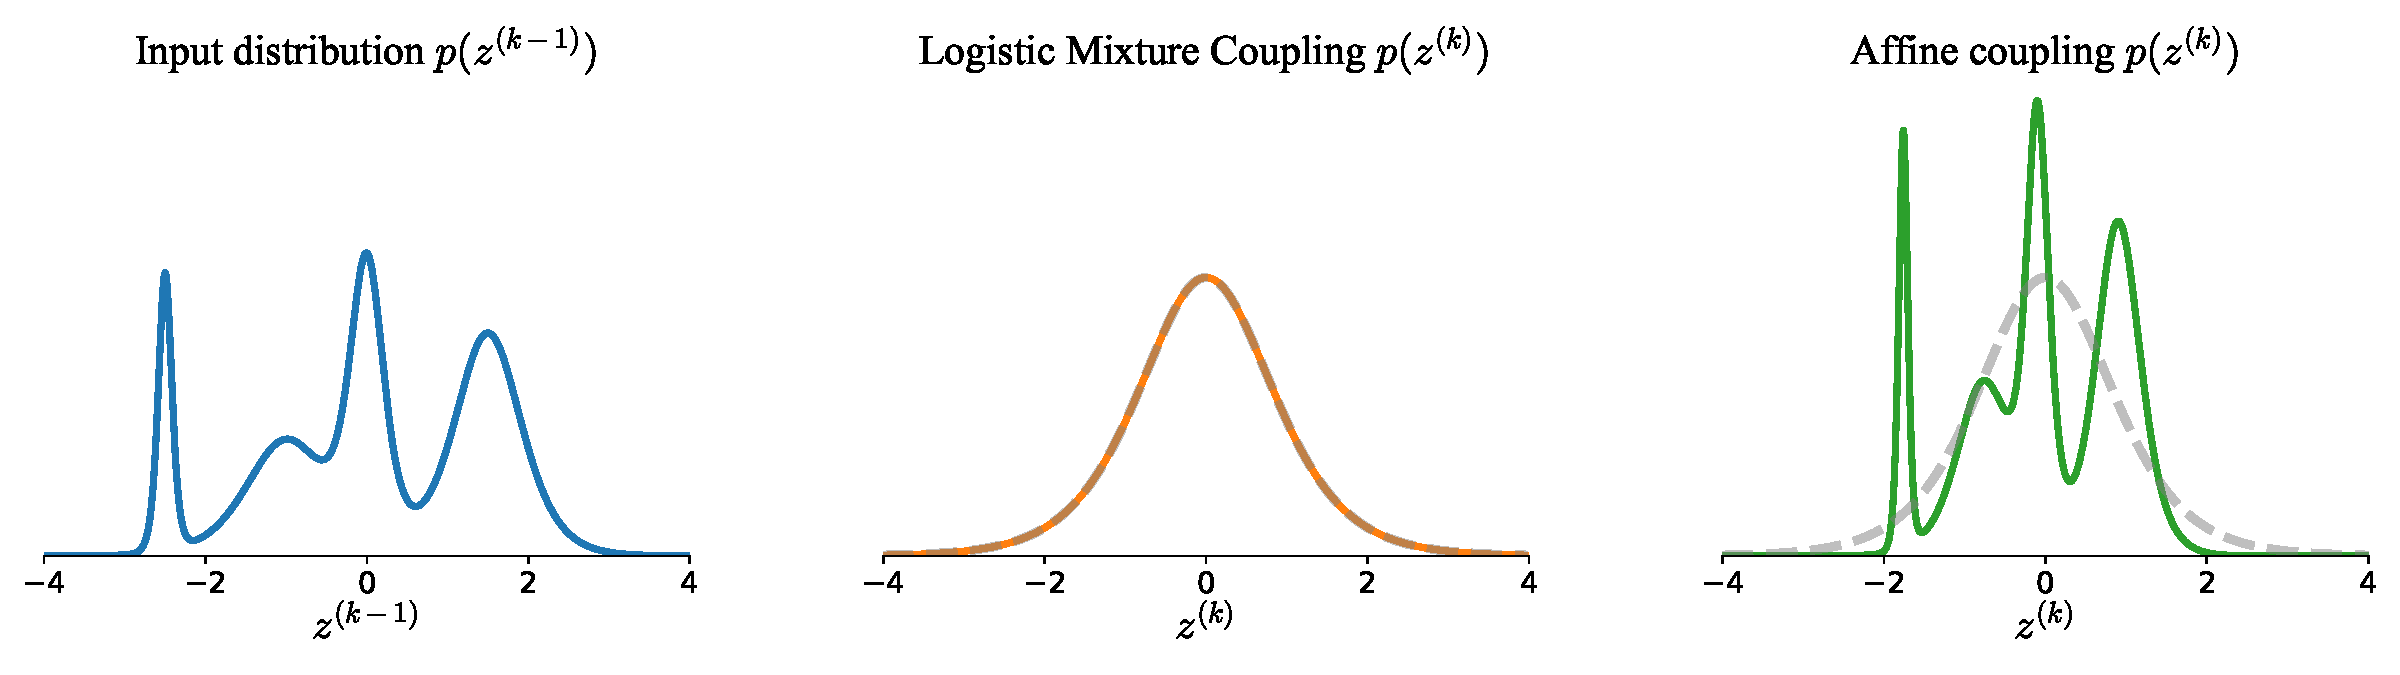
\includegraphics[width=\linewidth]{figures/flow_layer_figures/MoL_logistic_prior_font.pdf}
    \end{subfigure}
    \caption[Comparing affine and logistic mixture coupling layer on single dimension]{Comparing a standard affine coupling layer with a logistic mixture variant on transforming a mixture model to a single mode (shown in gray) in one dimension. While the logistic mixture layer is able to map the input distribution to a single mode, the affine coupling can only change the scaling and mean. Such transformations are crucial for flows as prior distributions have commonly a single mode.}
    \label{sec:background_comparing_coupling_layers}
\end{figure}

\paragraph{Logistic Mixture Coupling} The logistic mixture coupling layer is based on the idea of mapping a distribution of $K$ mixtures back into a single mode. This allows more complex transformations than affine coupling and can especially help for multi-modal input distribution, as visualized in Figure~\ref{sec:background_comparing_coupling_layers}.

The transformation $f$ consists of applying a \ac{CDF} for a mixture of $K$ logistic distributions on $\bm{z}^{(k-1)}_{j+1:d}$. This transformation is followed by an inverse sigmoid to ensure a globally existing inverse of the layer, and a standard affine transformation parameterized by $a$ and $b$. The position $\bm{\mu}$ and scale $\bm{s}$, as well as the mixture components $\pi_{1,...,K}$ of those $K$ logistics are also parameterized by a neural network with $\bm{z}^{(k-1)}_{1:j}$ as input. The full transformation for a single scalar latent variable $z$ with given parameters $\bm{\pi}, \bm{\mu}, \bm{s}, a, b$ is defined as follows:
\begin{equation}
    y = \sigma^{-1}\left(\sum_{i=1}^{K} \pi_i \sigma\left(\frac{z-\mu_i}{\exp(-s_i)}\right)\right)\cdot \exp(a)+b
\end{equation}
where $\sigma$ represents the sigmoid function: $\sigma(x)=\left(1+\exp(-x)\right)^{-1}$.
In general, this coupling layer is not limited to the logistic distribution and could be applied to any mixture model. However, logistics provide a cheap and differentiable \ac{CDF} making them attractive for backpropagation-based optimization. 
The Jacobian determinant can be efficiently calculated based on the probability density function of the logistics.
Inverting the transformation requires the usage of an iterative algorithm like the bisection method because it represents a monotonically increasing function without an analytical inverse.

\subsubsection{Autoregressive flows}
Intuitively, a single coupling layer is limited by the inter-variable interactions it can model as the transformations solely depend on one part of the input. 
Furthermore, the other part of the input is not changed at all requiring multiple coupling layers to be used.
A class of more complex flows that are flexible enough to model any probability distribution while still having a triangular Jacobian are \textit{autoregressive flows}. 
Instead of splitting the input into two parts, autoregressive flows define an order of the latent variables and use all previous elements to calculate the transformation parameters of the next variable:
\begin{eqnarray}
	\bm{z}^{(k)}_{j} & = & f\left(\bm{z}^{(k-1)}_{j};\hspace{1mm} \bm{\Theta}\left(\bm{z}^{(k-1)}_{1:j-1}\right)\right)
\end{eqnarray}
The transformation $f$ can use the same design choices as in coupling layers. 
Networks for modeling the transformation parameters are usually recurrent neural networks or masked feedforward networks which support autoregressive prediction \cite{MaskedAutoregressiveFlow}.
While the forward pass can be parallelized, inverting the flow requires a sequential execution as for calculating $\bm{z}^{(k-1)}_j$, the outputs $\bm{z}^{(k-1)}_{1:j-1}$ need to be determined first. 
Such a sequential calculation significantly slows down the sampling process for which the inverse is required. 
However, the flow could also be flipped such that the inverse is used during training and the forward for sampling. 
Those flows are called \textit{inverse autoregressive flows} \cite{InverseAutoregressiveFlows}, and trade fast sampling for slow density estimation.

\subsubsection{Activation Normalization}

When training deep normalizing flows, initialization must be done carefully as arbitrary transformations with large scaling and/or bias terms can introduce a very high initial KL divergence \cite{NormalizingFlowsOverview}. 
Taking inspiration from normalization layers in standard neural networks, \citet{RealNVP} proposed to apply batch normalization on the outputs of each flow. 
This layer improves the gradient signal throughout the flow and stabilizes scaling-based transformations while keeping the output distribution close to the prior. 
Nevertheless, batch normalization has shown to be noisy for small mini-batches.

As an alternative, \citet{Glow} proposed an \textit{activation normalization} layer which performs an affine transformation using a scale and bias parameter that can be shared across certain dimensions. 
Thereby, the parameters are initialized such that for a randomly selected batch of data, the latent variables after this layer have a zero mean and unit variance. 
Still, the scale and mean parameter are afterwards treated as trainable variables. 
Activation Normalization has shown to stabilize normalizing flows despite their simplicity and is being used in most \acl{SOTA} architectures \cite{Glow, Flow++, FloWaveNet, VFlow, EmielDequantization}.

\subsubsection{Permutation layers}
When using coupling layers, it is important to alternate the input split to allow transformations on all variables. 
This is usually done by permuting the latent variables $\bm{z}$ across a dimension. 
For instance, when modeling images, \citet{RealNVP} reversed the order of the channels before performing a coupling layer.
However, this permutation is predefined and fixed although it is not clear whether this is the optimal split of latent variables for all coupling layers.
To allow a permutation to be learned, \citet{Glow} proposed an invertible 1x1 convolution where the weight matrix is initialized as a random rotation matrix. 
Specifically, the transformation can be formulated as:
\begin{equation}
    \bm{z}^{(k)} = \bm{W}\bm{z}^{(k-1)}
\end{equation}
with $\bm{W}\in\mathbb{R}^{D\times D}$. 
Note that this operation is performed across the dimension that should be permuted (e.g. channels in images).
The transformation is invertible if $\bm{W}$ is invertible itself. 
To guarantee the invertibility of $\bm{W}$, \citet{Glow} suggest representing the weight matrix in its LU decomposition:
\begin{equation}
    \bm{W} = \bm{P}\bm{L}\left(\bm{U} + \text{diag}\left(\bm{s}\right)\right)
\end{equation}
where $\bm{P}$ is a permutation matrix, $\bm{L}$ is a lower triangular matrix with ones on the diagonal, and $\bm{U}$ an upper triangular matrix with zeros on the diagonal. 
The vector $\bm{s}$ is an additional scaling term based on which the Jacobian can be calculated. 
While $\bm{P}$ is fixed after initialization, $\bm{L}$, $\bm{U}$ and $\bm{s}$ are being optimized while enforcing the triangularity of the matrices.
With such a decomposition, the invertible 1x1 convolution enables the optimization of the permutation within a normalizing flow. 